% This is the Reed College LaTeX thesis template. Most of the work
% for the document class was done by Sam Noble (SN), as well as this
% template. Later comments etc. by Ben Salzberg (BTS). Additional
% restructuring and APA support by Jess Youngberg (JY).
% Your comments and suggestions are more than welcome; please email
% them to cus@reed.edu
%
% See http://web.reed.edu/cis/help/latex.html for help. There are a
% great bunch of help pages there, with notes on
% getting started, bibtex, etc. Go there and read it if you're not
% already familiar with LaTeX.
%
% Any line that starts with a percent symbol is a comment.
% They won't show up in the document, and are useful for notes
% to yourself and explaining commands.
% Commenting also removes a line from the document;
% very handy for troubleshooting problems. -BTS

% As far as I know, this follows the requirements laid out in
% the 2002-2003 Senior Handbook. Ask a librarian to check the
% document before binding. -SN

%%
%% Preamble
%%
% \documentclass{<something>} must begin each LaTeX document
\documentclass[12pt,twoside]{reedthesis}
% Packages are extensions to the basic LaTeX functions. Whatever you
% want to typeset, there is probably a package out there for it.
% Chemistry (chemtex), screenplays, you name it.
% Check out CTAN to see: http://www.ctan.org/
%%
\usepackage{graphicx,latexsym}
\usepackage{amsmath}
\usepackage{amssymb,amsthm}
\usepackage{longtable,booktabs,setspace}
\usepackage{chemarr} %% Useful for one reaction arrow, useless if you're not a chem major
\usepackage[hyphens]{url}
% Added by CII
\usepackage[hidelinks]{hyperref}
\usepackage{lmodern}
\usepackage{float}
\floatplacement{figure}{H}
% End of CII addition
\usepackage{rotating}

% Next line commented out by CII
%%% \usepackage{natbib}
% Comment out the natbib line above and uncomment the following two lines to use the new
% biblatex-chicago style, for Chicago A. Also make some changes at the end where the
% bibliography is included.
%\usepackage{biblatex-chicago}
%\bibliography{thesis}


% Added by CII (Thanks, Hadley!)
% Use ref for internal links
\renewcommand{\hyperref}[2][???]{\autoref{#1}}
\def\chapterautorefname{Chapter}
\def\sectionautorefname{Section}
\def\subsectionautorefname{Subsection}
% End of CII addition

% Added by CII
\usepackage{caption}
\captionsetup{width=5in}
% End of CII addition

% \usepackage{times} % other fonts are available like times, bookman, charter, palatino


% To pass between YAML and LaTeX the dollar signs are added by CII
\title{\textbf{\Huge{Numerical methods for stochastic volatility models: \\[20pt] Heston model}}}
\author{Fernando O. Teixeira}
% The month and year that you submit your FINAL draft TO THE LIBRARY (May or December)
<<<<<<< HEAD
\date{agosto 04, 2017}
=======
\date{agosto 06, 2017}
>>>>>>> 0cc9a872c82a0bf49d58ab2188bcc6596444cc17
\division{Applied Mathematics}
\advisor{Hugo de la Cruz}
%If you have two advisors for some reason, you can use the following
% Uncommented out by CII
% End of CII addition

%%% Remember to use the correct department!
\department{Mathematics}
% if you're writing a thesis in an interdisciplinary major,
% uncomment the line below and change the text as appropriate.
% check the Senior Handbook if unsure.
%\thedivisionof{The Established Interdisciplinary Committee for}
% if you want the approval page to say "Approved for the Committee",
% uncomment the next line
%\approvedforthe{Committee}

% Added by CII
%%% Copied from knitr
%% maxwidth is the original width if it's less than linewidth
%% otherwise use linewidth (to make sure the graphics do not exceed the margin)
\makeatletter
\def\maxwidth{ %
  \ifdim\Gin@nat@width>\linewidth
    \linewidth
  \else
    \Gin@nat@width
  \fi
}
\makeatother

\renewcommand{\contentsname}{Table of Contents}
% End of CII addition

\setlength{\parskip}{0pt}

% Added by CII

\providecommand{\tightlist}{%
  \setlength{\itemsep}{0pt}\setlength{\parskip}{0pt}}

\Acknowledgements{
I want to thank a few people.
}

\Dedication{
You can have a dedication here if you wish.
}

\Preface{

}

\Abstract{
The preface pretty much says it all. \par  Second paragraph of abstract
starts here.
}

	\usepackage{amsthm}
	\usepackage{cancel}
	\graphicspath{ {figure/} }
% End of CII addition
%%
%% End Preamble
%%
%

\usepackage{amsthm}
\newtheorem{theorem}{Theorem}[section]
\newtheorem{lemma}{Lemma}[section]
\theoremstyle{definition}
\newtheorem{definition}{Definition}[section]
\newtheorem{corollary}{Corollary}[section]
\newtheorem{proposition}{Proposition}[section]
\theoremstyle{definition}
\newtheorem{example}{Example}[section]
\theoremstyle{remark}
\newtheorem*{remark}{Remark}
\begin{document}

% Everything below added by CII
      \maketitle
  
  \frontmatter % this stuff will be roman-numbered
  \pagestyle{empty} % this removes page numbers from the frontmatter
      \begin{acknowledgements}
      I want to thank a few people.
    \end{acknowledgements}
  
      \hypersetup{linkcolor=black}
    \setcounter{tocdepth}{2}
    \tableofcontents
  
      \listoftables
  
      \listoffigures
      \begin{abstract}
      The preface pretty much says it all. \par  Second paragraph of abstract
      starts here.
    \end{abstract}
      \begin{dedication}
      You can have a dedication here if you wish.
    \end{dedication}
  \mainmatter % here the regular arabic numbering starts
  \pagestyle{fancyplain} % turns page numbering back on

  \chapter{\texorpdfstring{altadvisor: `Your Other
  Advisor'}{altadvisor: Your Other Advisor}}\label{altadvisor-your-other-advisor}
  
  \chapter{Literature Review}\label{lt-review}
  
  This chapter presents the concepts of stochastic calculus, from the
  historic conception of how it first arose through the basic principles
  and applications in finance. More precisely, we address the classical
  Black-Scholes model and its limitations and the Heston model. This model
  is also well known, it introduces the concept of stochastic volatility
  which brings us closer to reality.
  
  \section{Stochastic Calculus}\label{stochastic-calculus}
  
  Stochastic calculus arises from stochastic processes and allows the
  creation of a theory of integration where both the integrand and
  integrator terms are stochastic processes. Stochastic calculus was
  created by the Japanese mathematician Kiyosi
  Itô\textasciitilde{}\footnote{There is another important stochastic integral, called the \textit{Stratonovich Integral} that unlike the Itô's integral, respects the conventional calculus chain rule. Also, the integral is evaluated at the interval's midpoint, instead of its left extreme.}
  in the 1940s and 1950s and is used for modelling financial options and
  in another wide variety of fields {[}1{]}. In this chapter we present
  the historical contexts in which the tools and models used arise, but
  our focus is introducing the concepts and notations that will be further
  used in our work.
  
  \subsection{Brownian Motion}\label{brownian-motion}
  
  The Brownian motion is the name given to the irregular motion observed
  in the motion of pollen particles suspended in fluid resulting from
  particle collision with atoms or molecules. It is named after Robert
  Brown, the first to have observed the movement in 1828. He noted two
  characteristic in the pollen movement {[}1{]}:
  \begin{itemize}
  \item
    the path of a given particle is very irregular, having a tangent at no
    point
  \item
    the motion of two distinct particles appear to be independent
  \end{itemize}
  The first quantitative works in brownian motion come from an interest in
  stock price fluctuation by Bachelier in 1900. Albert Einstein also
  leaned over the subject and in 1905 derived the transition density for
  Brownian motion from molecular-kinetic theory of heat {[}1,2{]}.
  
  In 1923, the Wiener process was coined in honor of Norbert Wiener
  mathematical proof of existence of the brownian motion and stating its
  properties as follows {[}3{]}:
  \begin{itemize}
  \item
    \(W_{0}=0\)
  \item
    The change in \(W\), given by \(\Delta W = W_{t+1}-W_{t}\), is
    normally distributed with mean zero and standard deviation
    \(\sqrt{\Delta t}\), meaning that
    \(\Delta W = \epsilon\sqrt{\Delta t}\), where \(\epsilon\) is
    \(N(0,1)\).
  \item
    If the increment \(\Delta t_1\) does not overlap with the time
    increment \(\Delta t_2\), then \(\Delta W_1\) and \(\Delta W_2\) are
    independent.
  \item
    The process is continuous, meaning that there are no jumps in the
    process.
  \item
    The process is a Markov process. This means that the conditional
    expectation of \(W_{t+1}\) given its entire history is equal to the
    conditional expectation of \(W_{t+1}\) given today's information. This
    can be written as: \(E[W_{t+1}|W_1, ..., W_t] = E[W_{t+1}|W_t]\).
  \item
    Consider the time interval \([0,t]\) with \(n\) equally spaced
    intervals given by \(t_i = \frac{it}{n}\). Then the paths of the
    Brownian motion have unbounded variation, this means that they are not
    differentiable and go towards infinity as \(n\) increases. The
    quadratic variation is given by
    \(\sum_{i=1}^{n}{(Z_{t_i}-Z_{t_{i-1}})^2} \rightarrow t\), meaning
    that when \(n\) increases it stays constant at \(t\). \ref{fig:wiener}
  \end{itemize}
  \begin{figure}
  
  {\centering 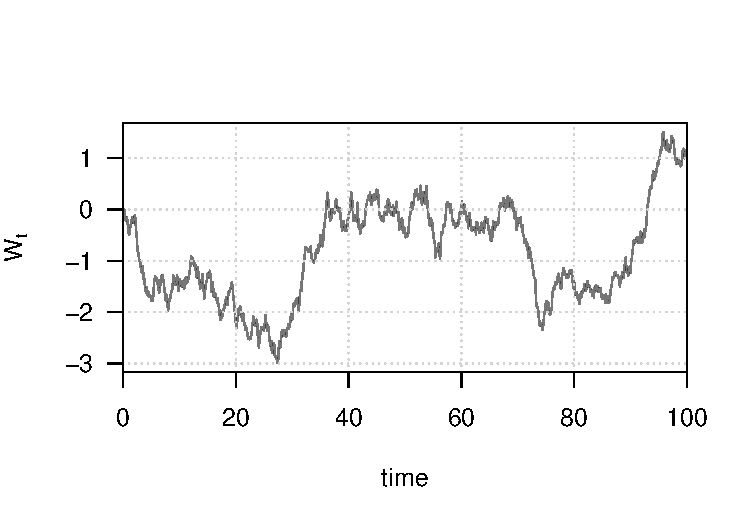
\includegraphics{thesis_files/figure-latex/wiener-1} 
  
  }
  
  \caption{A Wiener trajectory path example}\label{fig:wiener}
  \end{figure}
  \subsection{Correlated Brownian Motions}\label{corr}
  
  Two independent brownian motions that are correlated can describe a new
  process \(Z_t\). Let \(W_1\) and \(W_2\) be these two \emph{independent}
  Brownian motions and let \(-1 \leq \rho \leq 1\) be a given number. For
  \(0 \leq t \leq T\) define the new process \(Z_t\) as {[}1{]}:
  \begin{align}
  \label{eq:corr_brow}
  Z_t = \rho W_{1,t} + \sqrt{1-\rho^2}W_{2,t}
  \end{align}
  \noindent
  This equation is a linear combination of independent normals at each
  timestep \(t\), so \(Z_t\) is normally distributed. It is proven that
  \(Z\) is a Brownian motion and that \(Z\) and \(W_{1,t}\) are correlated
  {[}1{]}.
  
  \subsection{Arithmetic Brownian
  Motion}\label{arithmetic-brownian-motion}
  
  The arithmetic brownian motion is defined in literature as being a
  random process (S) defined as follows {[}1{]}:
  \begin{align}
  dS_t = \mu dt + \sigma dB_t
  \end{align}
  \begin{center}or in integral form:\end{center}
  \begin{align}
  \int_{t=0}^{T} dS_t = \int_{t=0}^{T}{\mu dt} + \int_{t=0}^{T}{\sigma dB_t}
  \end{align}
  \noindent
  Where, \(\mu\) and \(\sigma\) are known and constant with
  \(\sigma > 0\). In this process, both the drift \(\mu\) and the
  diffusion \(\sigma\) coefficient are constant. The expected value of
  this process is the sum of the initial value and the drift times the
  elapsed period (\(S_0 + \mu T\)). The variance is described by
  \(\sigma^2 T\)
  
  \subsection{Geometric Brownian Motion}\label{geometric-brownian-motion}
  
  A stochastic process \(S_t\) is a geometric brownian motion if its
  solution is described by the solution of the following stochastic
  differential equation {[}4,5{]}.
  \begin{align}
  dS_t = \mu S_t dt + \sigma S_t dW_t
  \end{align}
  \noindent
  for given constants \(\mu \in {\rm I\!R}\) and \(\sigma > 0\). Also, the
  assumed initial value is positive, \(S_0 >0\).
  
  This process is used quite often in finance to model the dynamics of
  some assets becaus of its properties. It has independent multiplicative
  increments and its solution is presented below{[}6{]}:
  \begin{align}
  S_t = S_0 \times exp{\left(\mu - \frac{\sigma^2}{2} \right) t + \sigma W_t}, \;\; t > 0
  \end{align}
  \subsection{Itô's Calculus}\label{itos-calculus}
  
  Let \(X_{t}\) be a real-valued stochastic process that satisfies
  {[}4,7,8{]}:
  \begin{align}
  S_t = S_0 + \int_{0}^{t} \mu_t dt + \int_{0}^{t} \sigma_t dW_t
  \end{align}
  \noindent
  for some \(\mu_t\), \(\sigma_t\) and \(t \in [0,T]\). This equation is
  often rewritten in its differential stochastic form:
  \begin{align}
  dS_t = \mu_t dt + \sigma_t dW_t 
  \end{align}
  \noindent
  for \(0 \leq t \leq T\).
  \begin{theorem}[Itô's Lemma]
  Assume that $S_t$ has a stochastic differential given by:
  \begin{align}
  dS_t = \mu_t dt + \sigma_t dW_t 
  \end{align}
  \noindent
  for $\mu_t$, $\sigma_t$ and $t \in [0,T]$. Assume $u: \mathbb{R} \times [0, T] \rightarrow \mathbb{R}$ is continuous and that $\frac{\partial u}{\partial t}$, $\frac{\partial u}{\partial x}$, $\frac{\partial^2 u}{\partial x^2}$ exist and are continuous.
  
  $$Y_t := u(S_t, t)$$
  \noindent
  Then Y has the following stochastic differential:
  \begin{align} 
  \label{eq:ito}
  \begin{split}
      dY_t &= \frac{\partial u}{\partial t}dt + \frac{\partial u}{\partial x} dS_t + \frac{1}{2}\frac{\partial^2 u}{\partial x^2}\sigma_t^2 dt  \\[10pt] 
      &= \left( \frac{\partial u}{\partial t} + \mu_t \frac{\partial u}{\partial x} + \frac{1}{2}\frac{\partial^2 u}{\partial x^2}\sigma_t^2 \right) dt + \sigma_t \frac{\partial u}{\partial x} dW_t
  \end{split}
  \end{align}
  \noindent 
  where the argument of $u$, $\frac{\partial u}{\partial x}$ and $\frac{\partial^2 u}{\partial x^2}$ above is $\left( S_t, t \right)$ .
  \end{theorem}
  \subsubsection{Getting to the Formula}\label{getting-to-the-formula}
  \begin{align}
  dS_t = \mu S_t dt + \sqrt{V_t} S_t dB_t
  \end{align}
  If \(S\) were deterministic, \(dS_t/S_t\) would be the derivative of
  \(\ln(S_t)\) with respect to \(S\). This suggests to find an expression
  for the stochastic differential of \(\ln(S_t)\), a function of the
  single random variable \(S_t\).
  \begin{scriptsize}
  \begin{align}
  f(t,S) &= \ln(S) \\
  df(t,S) &= \cancelto{0}{\frac{\partial f}{\partial t}dt}  + \frac{\partial f}{\partial S} dS + \cancelto{0}{\frac{1}{2} \frac{\partial^2 f}{\partial t^2} (dt)^2} + \frac{1}{2} \frac{\partial^2 f}{\partial S^2} (dS)^2  + \cancelto{0}{\frac{\partial^2 f}{\partial t \partial S} dt dS} \\
  d\ln(S) &= \frac{d\ln(S)}{dS} dS + \frac{1}{2} \frac{d^2\ln(S)}{dS^2}(dS)^2 \\
  (dS)^2 &= \int_{0}^{t}{\left(\sqrt{V} \times S \right)^2} ds = V S^2 dt \\
  d\ln(S) &= \frac{1}{S} (\mu S dt + \sqrt{V} S dB) + \frac{1}{2}\frac{-1}{S^2} V S^2 dt \\
  d\ln(S) &= \left( \mu -  \frac{1}{2} V \right) dt + \sqrt{V} dB \\
  \int_{u}^{T}{d\ln(S)} &= \int_{u}^{T}{\left( \mu - \frac{1}{2} V_t \right) dt} + \int_{u}^{T}{\sqrt{V_t}dB_t} \\
  \ln(S_t) - \ln(S_u) &= \int_{u}^{T}{\left( \mu - \frac{1}{2} V_t \right) dt} + \int_{u}^{T}{\sqrt{V_t}dB_t} \\
  \ln \left( \frac{S_t}{S_u} \right) &= \mu (t-u) - \frac{1}{2}\int_{u}^{T}{V_t dt} + \int_{u}^{T}{\sqrt{V_t} dB_t} \\
  \ln \left( \frac{S_t}{S_u} \right) &= \mu (t-u) - \frac{1}{2}\int_{u}^{T}{V_t dt} + \int_{u}^{T}{\sqrt{V_t} \left(\rho dB_{1,s} + \sqrt{1-\rho^2} dB_{1,s} \right)} \\
  S_t &= S_u \times \exp \left( \mu (t-u) - \frac{1}{2} \int_{u}^{T}{V_t dt} + \rho \int_{u}^{T}{\sqrt{V_t}dB_{1,t}}+ \sqrt{1 - \rho^2} \int_{u}^{T}{\sqrt{V_t}dB_{2,t}} \right)
  \end{align}
  \end{scriptsize}
  Equation \eqref{eq:ito} is the stochastic equivalent to the chain rule,
  also known as Itô's formula or Itô's chain rule. The proof to this
  theorem is based on the Taylor expansion of the function \(f(S_t, t)\)
  {[}4,7{]}. For practical uses you should write out a second-order Taylor
  expansion for the function to be analyzed and apply the
  \ref{tab:box-calc} multiplication table {[}1{]}.
  \begin{longtable}[t]{llr}
  \caption{\label{tab:box-calc}Box calculus}\\
  \toprule
    & $dt$ & $dW_t$\\
  \midrule
  $dt$ & 0 & 0\\
  $dW_t$ & 0 & $dt$\\
  \bottomrule
  \end{longtable}
  \section{Stochastic Differential Equations
  (SDE's)}\label{stochastic-differential-equations-sdes}
  
  \section{Black-Scholes Model}\label{black-scholes-model}
  
  The Black-Scholes (B-S) model arises from the need to price european
  options in the derivative markets. Derivatives are financial instruments
  traded in the market, stock exchange or over-the-counter (OTC) market,
  whose values depend on the values of an underlying asset. {[}9--11{]}
  \begin{itemize}
  \item
    A call option is a derivative that gives its bearer the right, but not
    the obligation, to purchase a specific asset by a fixed price before
    or on a given date.
  \item
    A put option is a derivative that gives its bearer the right, but not
    the obligation, to sell a specific asset by a fixed price before or on
    a given date.
  \end{itemize}
  The trading price of the option is called the option \emph{premium} and
  the asset from which the option derives is called the \emph{underlying
  asset}. This asset may be the interest rate, exchange rates, stock
  exchanges rates, commodities or stocks. The fixed price in contract in
  which the underlying asset might to be bought or sold is the
  \emph{strick price}. The option expiration date is called the
  \emph{maturity}. {[}10,11{]}
  
  There are two major different option types: the European and the
  American. The difference between these two is that the bearer of the
  first may exercise it only at the end of its life, at its maturity while
  the latter can be exercised at any given time until its maturity.
  {[}11,12{]}
  
  \subsection{The model}\label{the-model}
  
  The Black-Scholes model that provides analytical solution to the price
  of a European call at time \(t\) can be described as
  follows{[}3,9,11{]}:
  \begin{align}
  C(S_{t},t)&=N(d_{1})S_{t}-N(d_{2})Ke^{-r(T-t)}\\[10pt]
  d_{1}&={\frac {1}{\sigma {\sqrt {T-t}}}}\left[\ln \left({\frac {S_{t}}{K}}\right)+\left(r+{\frac {\sigma ^{2}}{2}}\right)(T-t)\right]\\[10pt]
  d_{2}&=d_{1}-\sigma {\sqrt {T-t}}
  \end{align}
  \noindent
  Where:
  \begin{itemize}
  \tightlist
  \item
    \(S_{t}\) is the spot price of the underlying asset at time \(t\)
  \item
    \(r\) is the risk free rate (generally an annual
    rate)\footnote{Assumed to be constant. \label{teste}}
  \item
    \(\sigma\) is the volatility of returns of the underlying asset
    \footnote{See footnote 1.}
  \item
    \(N(\cdot )\) is the cumulative distribution function of the standard
    Gaussian distribution
  \item
    \(K\) is the strike price
  \item
    \(T-t\) is the time to maturity
  \end{itemize}
  \noindent
  Also, the stock price path is a Geometric Brownian Motion and is under
  the risk-neutral measure with the following dynamics {[}3,13{]}:
  \begin{align}
  dS_{t} = (r-q)S_td_t+\sigma S_t dW_t
  \end{align}
  \noindent
  Where \(dW_t\) is a Wiener process {[}11,13{]}, \(r\) is the risk free
  rate and \(q\) is the dividend
  yield\footnote{$r$ and $q$ are assumed to be constant.} and \(t\)
  denotes the current point in time.
  
  Although the Black-Scholes is very popular and the \emph{de facto}
  standard in the market there are implications to the B-S model
  assumptions that affect the results and that are unrealistic. The main
  assumption that does not hold up is the deterministic (constant)
  volatility, that can more accurately be described as a stochastic
  process since we observe that small moves usually are followed by small
  moves and large moves by large moves. {[}3,9{]}
  
  Other assumptions that are critical to the B-S model and are not always
  observed in practice refer to the asset's continuity through time (no
  jumps), being allowed to perform continuous hedge without transactions
  costs and normal (Gaussian) returns.
  
  Most models focus on the volatility problem because transaction costs
  often translate to rises in volatility and fat-tails (abnormal) returns
  can be simulated by stochastic volatility and market or volatility
  jumps.
  
  \subsection{Limitations}\label{limitations}
  
  \section{Stochastic Volatility
  models}\label{stochastic-volatility-models}
  
  Introducing stochastic volatility to models brings complexity, but
  enables modeling some features observed in reality that are crucial like
  the randomic market volatility effects, skewness (market returns are
  more realistically modeled) and volatility smile. This kind of model is
  applied highly succesfully in foreign exchange and credit markets.
  
  \subsection{Other models (PRESENT MODELS PREVIOUSLY
  USED)}\label{other-models-present-models-previously-used}
  
  \subsection{Cox-Ingersoll-Ross model}\label{cox-ingersoll-ross-model}
  
  The Cox-Ingersoll-Ross (CIR) model is a well-known short-rate model that
  describes the interest rate movements driven by one source of market
  risk. The dynamics are described as follows{[}14,15{]}:
  \begin{align}
  \label{eq:cir}
  dr_t &= k(\theta - r_t)dt + \sigma \sqrt{r_t} dB_t
  \end{align}
  \noindent
  Where, \(r_t\) is the short rate interest described by parameters \(k\)
  - the speed of mean reversion, \(\theta\) - the long-run mean variance
  and \(\sigma\) - the volatility of the variance process.
  
  This model has been widely used to describe the dynamics of the short
  rate interest because it has some fundamental features like intuitive
  parametrization, nonnegativity and pricing formulas. Besides, it takes
  account of anticipations, risk aversion, investment alternatives and
  preferences about consumption timing and allows for detailed predictions
  about how changes in a wide range of underlying variables affect the
  term structure{[}14{]}. Furthermore, this equation constitutes one of
  the two Heston model equations with the volatility taking the short rate
  interest place.
  
  \subsection{Heston Model}\label{heston-model}
  
  Heston model solves the deterministic volatility problems introducing
  the following equations, which represents the dynamics of the stock
  price and the variance processes under the risk-neutral measure
  {[}15,16{]}:
  \begin{align}
  \label{eq:heston}
  \begin{split}
  dS_t &= \mu S_t dt + \sqrt{V_t} S_t dW^*_t \\
  dV_t &= k(\theta - V_t)dt + \sigma \sqrt{V_t} dB_t
  \end{split}
  \end{align}
  The second equation, as previously described, is the CIR model equation.
  The first equation states the asset price process. \(\mu\) is the
  asset's rate of return, \(dW_{t,1}\) and \(dW_{t,2}\) are two correlated
  wiener processes with correlation coefficient of \(\rho\). Because, of
  the model specifications and what we presentend in section \ref{corr},
  we can rewrite the first equation as in Broadie and Kaya {[}17{]}:
  \begin{align}
  \label{eq:heston2}
  \begin{split}
  dS_t &= \mu S_t dt + \rho \sqrt{V_t} dB_t + \sqrt{1 - \rho^2} \sqrt{V_t} S_t dW_t \\
  dV_t &= k(\theta - V_t)dt + \sigma \sqrt{V_t} dB_t
  \end{split}
  \end{align}
  \chapter{The Heston Model
  Implementation}\label{the-heston-model-implementation}
  
<<<<<<< HEAD
  \section{Characteristic Function}\label{characteristic-function}
  
  The Heston model characteristic function is firstly presented in the
  1993 Steven Heston's paper {[}15{]} and is described below {[}18{]}:
  \begin{align}
  f(S_t, V_t, t) = e^{A(T-t)+B(T-t)S_t + C(T-t)V_t + i \phi S_t}
  \end{align}
  If we let \(\tau = T-t\), then the explicit form of the Heston
  characteristic function is:
  \begin{align*}
  f(i \phi) &= e^{A(\tau)+B(\tau)S_t + C(\tau)V_t + i \phi S_t} \\
  A(\tau) &= r i \phi \tau + \frac{k \theta}{\sigma^2} \left[ - (\rho \sigma i \phi - k - M) \tau - 2 \ln\left(\frac{1-N e^{M \tau}}{1-N}\right) \right] \\
  B(\tau) &= 0 \\
  C(\tau) &= \frac{(e^{M \tau}-1)(\rho \sigma i \phi - k - M)}{\sigma^2 (1-N e^{M \tau})} \\
  \text{Where:} & \\
  M &= \sqrt{(\rho \sigma i \phi - k)^2 + \sigma^2 (i \phi + \phi^2)} \\
  N &= \frac{\rho \sigma i \phi - k - M}{\rho \sigma i \phi - k + M} \\
  \end{align*}
  This function is the driving force behind the following formula, that
  calculates the fair valur of a European call option at time \(t\), given
  a strike price \(K\), that expires at time \(T\) {[}18{]}:
  \begin{align} 
  \label{eq:cfheston}
  \begin{split}
  C = & \frac{1}{2} S(t) + \frac{e^{-r(T-t)}}{\pi}\int_{0}^{\infty}{\Re \left[ \frac{K^{-i \phi} f(i \phi + 1)}{i \phi} \right] d\phi} \\
  & -Ke^{-r(T-t)}\left( \frac{1}{2} + \frac{1}{\pi} \int_{0}^{\infty}{\Re \left[ \frac{K^{-i \phi} f(i \phi)}{i \phi} \right]}  d\phi \right)
  \end{split}
  \end{align}
  \section{Euler Scheme - Full
  Truncation}\label{euler-scheme---full-truncation}
  
  We present here the Euler Scheme - Full Truncation algorithm {[}17{]}
  along with some insights on how it was implemented in the R programming
  language {[}19{]}. The Euler discretization brings approximation paths
  to stock prices and variance processes. If we set
  \(t_0 = 0 < t_1 < \dots < t_M = T\) as partitions of a time interval of
  \(M\) equal segments of lenght \(\delta t\), we have the following
  discretization for the stock price:
  \begin{align}
  S_{t+1} = S_t + rS_t + \sqrt{V_t} S_t Z_s
  \end{align}
  \noindent
  And for the variance process:
  \begin{align}
  V_{t+1} = V_t + k (\theta - V_t) + \sigma \sqrt{V_t} Z_v
  \end{align}
  \noindent
  \(Z_s\) being a standard normal random variable, i.e. \(N~(0,1)\), we
  set \(Z_t\) and \(Z_v\) as two independent standard normal random
  variables and \(Z_s\) and \(Z_v\) having correlation \(\rho\). This
  means we can write \(Z_s = \rho Z_v + \sqrt{1-\rho^2} Z_t\)
  
  The immediate observable problem in the proposed discretization scheme
  is that \(V\) can become negative with non-zero probability making the
  computation of \(\sqrt{V_t}\) impossible {[}20{]}. There are several
  proposed fixes that can be used, we chose the Full-Truncation (FT) and
  rewrite the equations as follows:
  \begin{align}
  S_{t+1} &= S_t + rS_t + \sqrt{V_{t}^{+}} S_t Z_s \\
  V_{t+1} &= V_t + k (\theta - V_{t}^{+}) + \sigma \sqrt{V_{t}^{+}} Z_v
  \end{align}
  \noindent
  Where we use the notation \(V_{t}^{+} = \max(V_{t}, 0)\).
  \begin{Shaded}
  \begin{Highlighting}[]
  \NormalTok{hestoneuler <-}\StringTok{ }\ControlFlowTok{function}\NormalTok{(S, X, r, v, theta, rho, k, sigma, }\DataTypeTok{t =} \DecValTok{0}\NormalTok{, }
                          \DataTypeTok{dt =} \OtherTok{NULL}\NormalTok{, }\DataTypeTok{tau =} \DecValTok{1}\NormalTok{, N, }\DataTypeTok{sensibility =} \DecValTok{15}\NormalTok{)\{}
  
      \KeywordTok{set.seed}\NormalTok{(}\DecValTok{1}\NormalTok{)}
  
      \ControlFlowTok{if}\NormalTok{(}\KeywordTok{is.null}\NormalTok{(dt))\{ dt <-}\StringTok{ }\NormalTok{(tau}\OperatorTok{-}\NormalTok{t)}\OperatorTok{/}\DecValTok{1000}\NormalTok{\}}
  
  \NormalTok{    ST <-}\StringTok{ }\OtherTok{NULL}
  \NormalTok{    aux <-}\StringTok{ }\OtherTok{NULL}
  \NormalTok{    sqrt_dt <-}\StringTok{ }\KeywordTok{sqrt}\NormalTok{(dt)}
  
      \ControlFlowTok{for}\NormalTok{(i }\ControlFlowTok{in} \KeywordTok{seq}\NormalTok{(t,tau,dt))\{}
          \CommentTok{# browser()}
  \NormalTok{        Zv <-}\StringTok{ }\KeywordTok{rnorm}\NormalTok{(N)}
  \NormalTok{        Zt <-}\StringTok{ }\KeywordTok{rnorm}\NormalTok{(N)}
  \NormalTok{        Zs <-}\StringTok{ }\NormalTok{rho }\OperatorTok{*}\StringTok{ }\NormalTok{Zv }\OperatorTok{+}\StringTok{ }\NormalTok{(}\KeywordTok{sqrt}\NormalTok{(}\DecValTok{1} \OperatorTok{-}\StringTok{ }\NormalTok{(rho}\OperatorTok{^}\DecValTok{2}\NormalTok{)) }\OperatorTok{*}\StringTok{ }\NormalTok{Zt)}
  
          \CommentTok{# v[v <= 0] = 0}
  
  \NormalTok{        aux <-}\StringTok{ }\NormalTok{v}
  \NormalTok{        aux[v }\OperatorTok{<}\StringTok{ }\DecValTok{0}\NormalTok{] <-}\StringTok{ }\DecValTok{0}
  \NormalTok{        sqrt_aux <-}\StringTok{ }\KeywordTok{sqrt}\NormalTok{(aux)}
  \NormalTok{        S <-}\StringTok{ }\NormalTok{S }\OperatorTok{*}\StringTok{ }\NormalTok{(}\DecValTok{1} \OperatorTok{+}\StringTok{ }\NormalTok{r }\OperatorTok{*}\StringTok{ }\NormalTok{dt }\OperatorTok{+}\StringTok{ }\NormalTok{sqrt_aux }\OperatorTok{*}\StringTok{ }\NormalTok{Zs }\OperatorTok{*}\StringTok{ }\NormalTok{sqrt_dt)}
  \NormalTok{        S[S }\OperatorTok{<=}\StringTok{ }\DecValTok{0}\NormalTok{] =}\StringTok{ }\DecValTok{0}
  
  \NormalTok{        v <-}\StringTok{ }\NormalTok{v }\OperatorTok{+}\StringTok{ }\NormalTok{k }\OperatorTok{*}\StringTok{ }\NormalTok{dt }\OperatorTok{*}\StringTok{ }\NormalTok{(theta }\OperatorTok{-}\StringTok{ }\NormalTok{aux) }\OperatorTok{+}\StringTok{ }
  \StringTok{          }\NormalTok{sigma }\OperatorTok{*}\StringTok{ }\NormalTok{sqrt_aux }\OperatorTok{*}\StringTok{ }\NormalTok{Zv }\OperatorTok{*}\StringTok{ }\NormalTok{sqrt_dt}
  
  \NormalTok{        ST <-}\StringTok{ }\KeywordTok{rbind}\NormalTok{(ST,S)}
  \NormalTok{    \}}
  
      \KeywordTok{rm}\NormalTok{(aux, v, Zv, Zt, Zs, S)}
  
  \NormalTok{    ST <-}\StringTok{ }\KeywordTok{as.matrix}\NormalTok{(ST, }\DataTypeTok{ncol=}\NormalTok{N)}
      \CommentTok{# matplot(graf, type = 'l')}
      \CommentTok{# abline(h=X, lwd=2, col='red')}
  \NormalTok{    media <-}\StringTok{ }\KeywordTok{c}\NormalTok{()}
  
      \ControlFlowTok{for}\NormalTok{ (j }\ControlFlowTok{in}\NormalTok{ (X}\OperatorTok{-}\NormalTok{sensibility)}\OperatorTok{:}\NormalTok{(X}\OperatorTok{+}\NormalTok{sensibility))\{}
  
  \NormalTok{        Result <-}\StringTok{ }\NormalTok{ST[}\KeywordTok{nrow}\NormalTok{(ST),] }\OperatorTok{-}\StringTok{ }\NormalTok{j}
  \NormalTok{        Result[Result }\OperatorTok{<=}\StringTok{ }\DecValTok{0}\NormalTok{] <-}\StringTok{ }\DecValTok{0}
  \NormalTok{        media <-}\KeywordTok{c}\NormalTok{(media, }\KeywordTok{mean}\NormalTok{(Result))}
  
  \NormalTok{    \}}
  
  \NormalTok{    media <-}\StringTok{ }\NormalTok{media }\OperatorTok{*}\StringTok{ }\KeywordTok{exp}\NormalTok{(}\OperatorTok{-}\NormalTok{r}\OperatorTok{*}\NormalTok{tau)}
      \CommentTok{# plot(media, ylab = "Call price", xlab = "Strike price")}
  
  \NormalTok{    Result <-}\StringTok{ }\NormalTok{ST[}\KeywordTok{nrow}\NormalTok{(ST),] }\OperatorTok{-}\StringTok{ }\NormalTok{X}
  \NormalTok{    Result[Result }\OperatorTok{<=}\StringTok{ }\DecValTok{0}\NormalTok{] =}\StringTok{ }\DecValTok{0}
  \NormalTok{    call =}\StringTok{ }\KeywordTok{mean}\NormalTok{(}\KeywordTok{exp}\NormalTok{(}\OperatorTok{-}\NormalTok{r}\OperatorTok{*}\NormalTok{tau)}\OperatorTok{*}\NormalTok{Result)}
  
  \NormalTok{    lista =}\StringTok{ }\KeywordTok{list}\NormalTok{(}\StringTok{'call'}\NormalTok{ =}\StringTok{ }\NormalTok{call, }\StringTok{'Result'}\NormalTok{ =}\StringTok{ }\NormalTok{Result, }
                   \StringTok{'Spot'}\NormalTok{ =}\StringTok{ }\NormalTok{ST, }\StringTok{'sensib'}\NormalTok{ =}\StringTok{ }\NormalTok{media)}
      \KeywordTok{return}\NormalTok{(lista)}
  \NormalTok{\}}
  \end{Highlighting}
  \end{Shaded}
  \section{Kahl-Jackel}\label{kahl-jackel}
  \begin{Shaded}
  \begin{Highlighting}[]
  \NormalTok{Hestoncallkj <-}\StringTok{ }\ControlFlowTok{function}\NormalTok{(S, X, r, q, v, theta, rho, k, sigma, }
                           \DataTypeTok{t =} \DecValTok{0}\NormalTok{, }\DataTypeTok{dt =} \OtherTok{NULL}\NormalTok{, }\DataTypeTok{tau =} \DecValTok{1}\NormalTok{, N, }
                           \DataTypeTok{sensibility =} \DecValTok{15}\NormalTok{)\{}
  
      \ControlFlowTok{if}\NormalTok{(}\KeywordTok{is.null}\NormalTok{(dt))\{ dt <-}\StringTok{ }\NormalTok{(T}\OperatorTok{-}\NormalTok{t)}\OperatorTok{/}\DecValTok{1000}\NormalTok{\}}
  
  \NormalTok{    v <-}\StringTok{ }\KeywordTok{rep}\NormalTok{(v,N)}
  \NormalTok{    theta<-}\StringTok{ }\KeywordTok{rep}\NormalTok{(theta,N)}
  \NormalTok{    graf <-}\StringTok{ }\OtherTok{NULL}
  \NormalTok{    S <-}\StringTok{ }\KeywordTok{log}\NormalTok{(S)}
  
      \ControlFlowTok{for}\NormalTok{(i }\ControlFlowTok{in} \KeywordTok{seq}\NormalTok{(t,tau,dt))\{}
       \CommentTok{# browser()}
  \NormalTok{    Zv <-}\StringTok{ }\KeywordTok{rnorm}\NormalTok{(N)}
  \NormalTok{    Zt <-}\StringTok{ }\KeywordTok{rnorm}\NormalTok{(N)}
  \NormalTok{    Zs <-}\StringTok{ }\NormalTok{rho }\OperatorTok{*}\StringTok{ }\NormalTok{Zv }\OperatorTok{+}\StringTok{ }\KeywordTok{sqrt}\NormalTok{(}\DecValTok{1} \OperatorTok{-}\StringTok{ }\NormalTok{rho}\OperatorTok{^}\DecValTok{2}\NormalTok{) }\OperatorTok{*}\StringTok{ }\NormalTok{Zt}
  
  \NormalTok{    vt <-}\StringTok{ }\NormalTok{(v }\OperatorTok{+}\StringTok{ }\NormalTok{k }\OperatorTok{*}\StringTok{ }\NormalTok{theta }\OperatorTok{*}\StringTok{ }\NormalTok{dt }\OperatorTok{+}\StringTok{ }\NormalTok{sigma }\OperatorTok{*}\StringTok{ }\KeywordTok{sqrt}\NormalTok{(v) }\OperatorTok{*}\StringTok{ }\NormalTok{Zv }\OperatorTok{*}\StringTok{ }\KeywordTok{sqrt}\NormalTok{(dt) }\OperatorTok{+}
  \StringTok{              }\NormalTok{(}\DecValTok{1}\OperatorTok{/}\DecValTok{4}\NormalTok{) }\OperatorTok{*}\StringTok{ }\NormalTok{sigma}\OperatorTok{^}\DecValTok{2} \OperatorTok{*}\StringTok{ }\NormalTok{dt }\OperatorTok{*}\StringTok{ }\NormalTok{((Zv)}\OperatorTok{^}\DecValTok{2} \OperatorTok{-}\StringTok{ }\DecValTok{1}\NormalTok{))}\OperatorTok{/}\NormalTok{(}\DecValTok{1} \OperatorTok{+}\StringTok{ }\NormalTok{k }\OperatorTok{*}\StringTok{ }\NormalTok{dt)}
  
      \CommentTok{# print(vt)}
  
      \CommentTok{# if(!length(vt[vt <= 0]) == 0 & length(vt[vt <= 0]) >= 1)\{}
      \CommentTok{#     # browser()}
  \NormalTok{    vt[vt }\OperatorTok{<=}\StringTok{ }\DecValTok{0}\NormalTok{] <-}\StringTok{ }\NormalTok{v[vt }\OperatorTok{<=}\StringTok{ }\DecValTok{0}\NormalTok{] }\OperatorTok{+}\StringTok{ }\NormalTok{k }\OperatorTok{*}\StringTok{ }\NormalTok{dt }\OperatorTok{*}\StringTok{ }\NormalTok{(theta[vt }\OperatorTok{<=}\StringTok{ }\DecValTok{0}\NormalTok{] }\OperatorTok{-}\StringTok{ }
  \StringTok{                    }\KeywordTok{pmax}\NormalTok{(v[vt }\OperatorTok{<=}\StringTok{ }\DecValTok{0}\NormalTok{],}\DecValTok{0}\NormalTok{)) }\OperatorTok{+}\StringTok{ }\NormalTok{sigma }\OperatorTok{*}\StringTok{ }
  \StringTok{                    }\KeywordTok{sqrt}\NormalTok{(}\KeywordTok{pmax}\NormalTok{(v[vt }\OperatorTok{<=}\StringTok{ }\DecValTok{0}\NormalTok{],}\DecValTok{0}\NormalTok{)) }\OperatorTok{*}\StringTok{ }\NormalTok{Zv[vt }\OperatorTok{<=}\StringTok{ }\DecValTok{0}\NormalTok{] }\OperatorTok{*}\StringTok{ }\KeywordTok{sqrt}\NormalTok{(dt)}
  \NormalTok{    v <-}\StringTok{ }\NormalTok{vt}
  \NormalTok{    v[v}\OperatorTok{<=}\DecValTok{0}\NormalTok{] <-}\StringTok{ }\DecValTok{0}
  
      \CommentTok{# \}}
  
  \NormalTok{    S <-}\StringTok{ }\NormalTok{S }\OperatorTok{+}\StringTok{ }\NormalTok{(r }\OperatorTok{-}\StringTok{ }\NormalTok{(v}\OperatorTok{+}\NormalTok{vt)}\OperatorTok{/}\DecValTok{4}\NormalTok{) }\OperatorTok{*}\StringTok{ }\NormalTok{dt }\OperatorTok{+}\StringTok{ }\NormalTok{rho }\OperatorTok{*}\StringTok{ }\KeywordTok{sqrt}\NormalTok{(}\KeywordTok{pmax}\NormalTok{(v,}\DecValTok{0}\NormalTok{)) }\OperatorTok{*}\StringTok{ }
  \StringTok{          }\NormalTok{Zv }\OperatorTok{*}\StringTok{ }\KeywordTok{sqrt}\NormalTok{(dt) }\OperatorTok{+}
  \StringTok{          }\NormalTok{(}\DecValTok{1}\OperatorTok{/}\DecValTok{2}\NormalTok{) }\OperatorTok{*}\StringTok{ }\NormalTok{(}\KeywordTok{sqrt}\NormalTok{(}\KeywordTok{pmax}\NormalTok{(v,}\DecValTok{0}\NormalTok{)) }\OperatorTok{+}\StringTok{ }\KeywordTok{sqrt}\NormalTok{(}\KeywordTok{pmax}\NormalTok{(vt,}\DecValTok{0}\NormalTok{))) }\OperatorTok{*}\StringTok{ }
  \StringTok{          }\NormalTok{(Zs }\OperatorTok{+}\StringTok{ }\NormalTok{rho }\OperatorTok{*}\StringTok{ }\NormalTok{Zv) }\OperatorTok{*}\StringTok{ }
  \StringTok{          }\KeywordTok{sqrt}\NormalTok{(dt) }\OperatorTok{+}
  \StringTok{          }\NormalTok{((rho }\OperatorTok{*}\StringTok{ }\NormalTok{sigma }\OperatorTok{*}\StringTok{ }\NormalTok{dt)}\OperatorTok{/}\DecValTok{2}\NormalTok{) }\OperatorTok{*}\StringTok{ }\NormalTok{((Zv)}\OperatorTok{^}\DecValTok{2} \OperatorTok{-}\StringTok{ }\DecValTok{1}\NormalTok{)}
  
  \NormalTok{    S[S }\OperatorTok{<=}\StringTok{ }\DecValTok{0}\NormalTok{] =}\StringTok{ }\DecValTok{0}
  \NormalTok{    graf <-}\StringTok{ }\KeywordTok{rbind}\NormalTok{(graf,S)}
  
  \NormalTok{    \}}
  
       \CommentTok{# browser()}
  
  \NormalTok{    graf <-}\StringTok{ }\KeywordTok{as.matrix}\NormalTok{(graf, }\DataTypeTok{ncol=}\NormalTok{N)}
  \NormalTok{    ST <-}\StringTok{ }\NormalTok{graf}
      \CommentTok{# matplot(graf, type = 'l')}
      \CommentTok{# abline(h=log(X), lwd=2, col='red')}
  
  \NormalTok{    media <-}\StringTok{ }\KeywordTok{c}\NormalTok{()}
  
      \CommentTok{# browser()}
  
      \ControlFlowTok{for}\NormalTok{ (j }\ControlFlowTok{in}\NormalTok{ (X}\OperatorTok{-}\NormalTok{sensibility)}\OperatorTok{:}\NormalTok{(X}\OperatorTok{+}\NormalTok{sensibility))\{}
  
  \NormalTok{        Result <-}\StringTok{ }\KeywordTok{exp}\NormalTok{(ST[}\KeywordTok{nrow}\NormalTok{(ST),]) }\OperatorTok{-}\StringTok{ }\NormalTok{j}
  \NormalTok{        Result[Result }\OperatorTok{<=}\StringTok{ }\DecValTok{0}\NormalTok{] <-}\StringTok{ }\DecValTok{0}
  \NormalTok{        media <-}\KeywordTok{c}\NormalTok{(media, }\KeywordTok{mean}\NormalTok{(Result))}
  
  \NormalTok{    \}}
  
  \NormalTok{    media <-}\StringTok{ }\NormalTok{media }\OperatorTok{*}\StringTok{ }\KeywordTok{exp}\NormalTok{(}\OperatorTok{-}\NormalTok{r}\OperatorTok{*}\NormalTok{tau)}
  
      \CommentTok{# browser()}
  
  \NormalTok{    Result <-}\StringTok{ }\KeywordTok{exp}\NormalTok{(ST[}\KeywordTok{nrow}\NormalTok{(ST),]) }\OperatorTok{-}\StringTok{ }\NormalTok{X}
  \NormalTok{    Result[Result }\OperatorTok{<=}\StringTok{ }\DecValTok{0}\NormalTok{] =}\StringTok{ }\DecValTok{0}
  \NormalTok{    call =}\StringTok{ }\KeywordTok{mean}\NormalTok{(}\KeywordTok{exp}\NormalTok{(}\OperatorTok{-}\NormalTok{r}\OperatorTok{*}\NormalTok{tau)}\OperatorTok{*}\NormalTok{Result)}
  
  \NormalTok{    lista =}\StringTok{ }\KeywordTok{list}\NormalTok{(}\StringTok{'call'}\NormalTok{ =}\StringTok{ }\NormalTok{call, }\StringTok{'Result'}\NormalTok{ =}\StringTok{ }\NormalTok{Result, }
                   \StringTok{'Spot'}\NormalTok{ =}\StringTok{ }\NormalTok{graf, }\StringTok{'sensib'}\NormalTok{ =}\StringTok{ }\NormalTok{media)}
      \KeywordTok{return}\NormalTok{(lista)}
  
  \NormalTok{\}}
  \end{Highlighting}
  \end{Shaded}
  \section{Exact Algorithm}\label{exact-algorithm}
  \begin{Shaded}
  \begin{Highlighting}[]
  \NormalTok{hestonea <-}\StringTok{ }\ControlFlowTok{function}\NormalTok{(S, X, r, v, theta, rho, k, sigma, }\DataTypeTok{t =} \DecValTok{0}\NormalTok{, }
                       \DataTypeTok{dt =} \OtherTok{NULL}\NormalTok{, }\DataTypeTok{tau =} \DecValTok{1}\NormalTok{, N, }\DataTypeTok{sensibility =} \DecValTok{15}\NormalTok{)\{}
  
      \ControlFlowTok{if}\NormalTok{(}\KeywordTok{is.null}\NormalTok{(dt))\{ dt <-}\StringTok{ }\NormalTok{(tau}\OperatorTok{-}\NormalTok{t)}\OperatorTok{/}\DecValTok{1000}\NormalTok{\}}
  
  \NormalTok{    ST <-}\StringTok{ }\OtherTok{NULL}
  
  \NormalTok{    d <-}\StringTok{ }\NormalTok{(}\DecValTok{4} \OperatorTok{*}\StringTok{ }\NormalTok{k }\OperatorTok{*}\StringTok{ }\NormalTok{theta)}\OperatorTok{/}\NormalTok{(sigma)}\OperatorTok{^}\DecValTok{2}
  \NormalTok{    c0 <-}\StringTok{ }\NormalTok{(sigma}\OperatorTok{^}\DecValTok{2} \OperatorTok{*}\StringTok{ }\NormalTok{(}\DecValTok{1} \OperatorTok{-}\StringTok{ }\KeywordTok{exp}\NormalTok{(}\OperatorTok{-}\NormalTok{k}\OperatorTok{*}\NormalTok{dt)))}\OperatorTok{/}\NormalTok{(}\DecValTok{4}\OperatorTok{*}\NormalTok{k)}
  
      \CommentTok{# browser()}
  
      \ControlFlowTok{for}\NormalTok{(i }\ControlFlowTok{in} \KeywordTok{seq}\NormalTok{(t,tau,dt))\{}
  
          \CommentTok{# sampling V}
  \NormalTok{        lambda <-}\StringTok{ }\NormalTok{(}\DecValTok{4}\OperatorTok{*}\NormalTok{k}\OperatorTok{*}\KeywordTok{exp}\NormalTok{(}\OperatorTok{-}\NormalTok{k}\OperatorTok{*}\NormalTok{dt)}\OperatorTok{*}\NormalTok{v)}\OperatorTok{/}\NormalTok{(sigma}\OperatorTok{^}\DecValTok{2} \OperatorTok{*}\StringTok{ }\NormalTok{(}\DecValTok{1}\OperatorTok{-}\KeywordTok{exp}\NormalTok{(}\OperatorTok{-}\NormalTok{k}\OperatorTok{*}\NormalTok{dt)))}
  \NormalTok{        vt <-}\StringTok{ }\NormalTok{c0 }\OperatorTok{*}\StringTok{ }\KeywordTok{rchisq}\NormalTok{(}\DataTypeTok{n =}\NormalTok{ N, }\DataTypeTok{df =}\NormalTok{ d, }\DataTypeTok{ncp =}\NormalTok{ lambda)}
  
          \CommentTok{# Sampling int\{V\}}
  \NormalTok{        int_v <-}\StringTok{ }\NormalTok{dt }\OperatorTok{*}\StringTok{ }\NormalTok{((}\DecValTok{1}\OperatorTok{/}\DecValTok{2}\NormalTok{) }\OperatorTok{*}\StringTok{ }\NormalTok{v }\OperatorTok{+}\StringTok{ }\NormalTok{(}\DecValTok{1}\OperatorTok{/}\DecValTok{2}\NormalTok{) }\OperatorTok{*}\StringTok{ }\NormalTok{vt)}
  
          \CommentTok{# Sampling int\{v\}dw}
  \NormalTok{        int_vdw <-}\StringTok{ }\NormalTok{(}\DecValTok{1}\OperatorTok{/}\NormalTok{sigma) }\OperatorTok{*}\StringTok{ }\NormalTok{(vt }\OperatorTok{-}\StringTok{ }\NormalTok{v }\OperatorTok{-}\StringTok{ }\NormalTok{k }\OperatorTok{*}\StringTok{ }\NormalTok{theta }\OperatorTok{*}\StringTok{ }\NormalTok{dt }\OperatorTok{+}\StringTok{ }\NormalTok{k  }\OperatorTok{*}\StringTok{ }\NormalTok{int_v)}
  
          \CommentTok{# Sampling S}
  \NormalTok{        m <-}\StringTok{ }\KeywordTok{log}\NormalTok{(S) }\OperatorTok{+}\StringTok{ }\NormalTok{(r }\OperatorTok{*}\StringTok{ }\NormalTok{dt }\OperatorTok{-}\StringTok{ }\NormalTok{(}\DecValTok{1}\OperatorTok{/}\DecValTok{2}\NormalTok{) }\OperatorTok{*}\StringTok{ }\NormalTok{int_v }\OperatorTok{+}\StringTok{ }\NormalTok{rho }\OperatorTok{*}\StringTok{ }\NormalTok{int_vdw)}
  \NormalTok{        std <-}\StringTok{ }\KeywordTok{sqrt}\NormalTok{((}\DecValTok{1} \OperatorTok{-}\StringTok{ }\NormalTok{rho}\OperatorTok{^}\DecValTok{2}\NormalTok{)) }\OperatorTok{*}\StringTok{ }\KeywordTok{sqrt}\NormalTok{(int_v)}
  \NormalTok{        S <-}\StringTok{ }\KeywordTok{exp}\NormalTok{(m }\OperatorTok{+}\StringTok{ }\NormalTok{std }\OperatorTok{*}\StringTok{ }\KeywordTok{rnorm}\NormalTok{(N))}
  \NormalTok{        v <-}\StringTok{ }\NormalTok{vt}
  \NormalTok{        ST <-}\StringTok{ }\KeywordTok{rbind}\NormalTok{(ST,S)}
  \NormalTok{    \}}
  
  \NormalTok{    ST <-}\StringTok{ }\KeywordTok{as.matrix}\NormalTok{(ST, }\DataTypeTok{ncol=}\NormalTok{N)}
      \CommentTok{# matplot(graf, type = 'l')}
      \CommentTok{# abline(h=X, lwd=2, col='red')}
  \NormalTok{    media <-}\StringTok{ }\KeywordTok{c}\NormalTok{()}
  
      \ControlFlowTok{for}\NormalTok{ (j }\ControlFlowTok{in}\NormalTok{ (X}\OperatorTok{-}\NormalTok{sensibility)}\OperatorTok{:}\NormalTok{(X}\OperatorTok{+}\NormalTok{sensibility))\{}
  
  \NormalTok{        Result <-}\StringTok{ }\NormalTok{ST[}\KeywordTok{nrow}\NormalTok{(ST),] }\OperatorTok{-}\StringTok{ }\NormalTok{j}
  \NormalTok{        Result[Result }\OperatorTok{<=}\StringTok{ }\DecValTok{0}\NormalTok{] <-}\StringTok{ }\DecValTok{0}
  \NormalTok{        media <-}\KeywordTok{c}\NormalTok{(media, }\KeywordTok{mean}\NormalTok{(Result))}
  
  \NormalTok{    \}}
  
  \NormalTok{    media <-}\StringTok{ }\NormalTok{media }\OperatorTok{*}\StringTok{ }\KeywordTok{exp}\NormalTok{(}\OperatorTok{-}\NormalTok{r}\OperatorTok{*}\NormalTok{tau)}
      \CommentTok{# plot(media, ylab = "Call price", xlab = "Strike price")}
  
  \NormalTok{    Result <-}\StringTok{ }\NormalTok{ST[}\KeywordTok{nrow}\NormalTok{(ST),] }\OperatorTok{-}\StringTok{ }\NormalTok{X}
  \NormalTok{    Result[Result }\OperatorTok{<=}\StringTok{ }\DecValTok{0}\NormalTok{] =}\StringTok{ }\DecValTok{0}
  \NormalTok{    call =}\StringTok{ }\KeywordTok{mean}\NormalTok{(}\KeywordTok{exp}\NormalTok{(}\OperatorTok{-}\NormalTok{r}\OperatorTok{*}\NormalTok{tau)}\OperatorTok{*}\NormalTok{Result)}
  
  \NormalTok{    lista =}\StringTok{ }\KeywordTok{list}\NormalTok{(}\StringTok{'call'}\NormalTok{ =}\StringTok{ }\NormalTok{call, }\StringTok{'Result'}\NormalTok{ =}\StringTok{ }\NormalTok{Result, }
                   \StringTok{'Spot'}\NormalTok{ =}\StringTok{ }\NormalTok{ST, }\StringTok{'sensib'}\NormalTok{ =}\StringTok{ }\NormalTok{media)}
      \KeywordTok{return}\NormalTok{(lista)}
  \NormalTok{\}}
  \end{Highlighting}
  \end{Shaded}
  \clearpage
  \begin{Shaded}
  \begin{Highlighting}[]
  \KeywordTok{require}\NormalTok{(NMOF)}
  \KeywordTok{setwd}\NormalTok{(}\StringTok{"../rnmethods"}\NormalTok{)}
  \KeywordTok{source}\NormalTok{(}\StringTok{"../rnmethods/R/euler_heston.R"}\NormalTok{)}
  \end{Highlighting}
  \end{Shaded}
  \chapter{Results}\label{results}
=======
  \chapter{This chunk ensures that the thesisdown package
  is}\label{this-chunk-ensures-that-the-thesisdown-package-is}
>>>>>>> 0cc9a872c82a0bf49d58ab2188bcc6596444cc17
  
  \chapter{Conclusion}\label{conclusion}
  
  \chapter{The First Appendix}\label{the-first-appendix}
  
  \chapter*{References}\label{references}
  \addcontentsline{toc}{chapter}{References}
  
  \hypertarget{refs}{}
  \hypertarget{ref-ubbo}{}
  {[}1{]} U.F. Wiersema, Brownian motion calculus, John Wiley \& Sons,
  2008.
  
  \hypertarget{ref-karatzas2012brownian}{}
  {[}2{]} I. Karatzas, S. Shreve, Brownian motion and stochastic calculus,
  Springer Science \& Business Media, 2012.
  
  \hypertarget{ref-helgadottir2016option}{}
  {[}3{]} A.D. Helgadóttir, L. Ionescu, Option pricing within the heston
  model, (2016).
  
  \hypertarget{ref-tong2012option}{}
  {[}4{]} Z. Tong, Option pricing with long memory stochastic volatility
  models, PhD thesis, Université d'Ottawa/University of Ottawa, 2012.
  
  \hypertarget{ref-tsay2005analysis}{}
  {[}5{]} R.S. Tsay, Analysis of financial time series, John Wiley \&
  Sons, 2005.
  
  \hypertarget{ref-iacus2009simulation}{}
  {[}6{]} S.M. Iacus, Simulation and inference for stochastic differential
  equations: With r examples, Springer Science \& Business Media, 2009.
  
  \hypertarget{ref-evans2012introduction}{}
  {[}7{]} L.C. Evans, An introduction to stochastic differential
  equations, American Mathematical Soc., 2012.
  
  \hypertarget{ref-steele2012stochastic}{}
  {[}8{]} J.M. Steele, Stochastic calculus and financial applications,
  Springer Science \& Business Media, 2012.
  
  \hypertarget{ref-yang2013valuing}{}
  {[}9{]} Y. Yang, Valuing a european option with the heston model,
  (2013).
  
  \hypertarget{ref-salomao2011precificaccao}{}
  {[}10{]} M. de F. Salomão, Precificação de opções financeiras: Um estudo
  sobre os modelos de black scholes e garch, (2011).
  
  \hypertarget{ref-black1973pricing}{}
  {[}11{]} F. Black, M. Scholes, The pricing of options and corporate
  liabilities, Journal of Political Economy. 81 (1973) 637--654.
  
  \hypertarget{ref-merton1973theory}{}
  {[}12{]} R.C. Merton, Theory of rational option pricing, The Bell
  Journal of Economics and Management Science. (1973) 141--183.
  
  \hypertarget{ref-nmof}{}
  {[}13{]} M. Gilli, D. Maringer, E. Schumann, Numerical methods and
  optimization in finance, Academic Press, Waltham, MA, USA, 2011.
  \url{http://nmof.net}.
  
  \hypertarget{ref-cox1985theory}{}
  {[}14{]} J.C. Cox, J.E. Ingersoll Jr, S.A. Ross, A theory of the term
  structure of interest rates, Econometrica: Journal of the Econometric
  Society. (1985) 385--407.
  
  \hypertarget{ref-heston1993closed}{}
  {[}15{]} S.L. Heston, A closed-form solution for options with stochastic
  volatility with applications to bond and currency options, Review of
  Financial Studies. 6 (1993) 327--343.
  
  \hypertarget{ref-gilli_numerical_2011}{}
  {[}16{]} M. Gilli, D. Maringer, E. Schumann, Numerical methods and
  optimization in finance, Academic Press, 2011.
  
  \hypertarget{ref-broadie2006exact}{}
  {[}17{]} M. Broadie, Ö. Kaya, Exact simulation of stochastic volatility
  and other affine jump diffusion processes, Operations Research. 54
  (2006) 217--231.


  % Index?

\end{document}
